\documentclass[ letterpaper,12pt]{article}

\usepackage[english]{babel}
\usepackage[T1]{fontenc}
\usepackage{a4wide}
\usepackage{graphicx}
\usepackage{epsfig}

\begin{document}

\title{\textbf{DccNiTghmare's Player Book}}

\author{
DccNiTghtmare\\ \& Anamabeka
}

\maketitle
\abstract{This document describes all (and some more) things about playable races and classes on DccNiTghtmare.}

\newpage

\tableofcontents

\newpage
\section{Introduction}

Welcome to DccNiTghtmare, a post-nuclear world of adventure and fantasy. In
this game you'll take control of an UFMG student, or from that university you
always dreamed about. In this game you can:

\begin{itemize}
\item{Search for treasures on teacher's room;}
\item{Change that bad score that you can't, by no means, recuperate;}
\item{Kill;}
\item{Plunder;}
\item{Destroy;}
\item{Walk armed in the campus;}
\item{Negotiate tests for biscuits;}
\item{Reach warp 3;}
\item{Recruit hordes to make the chaos with you;}
\item{Fight epic battles;}
\item{"Practice Free-Fight with a carnivorous gorilla" (sic);}
\item{Train battle ameivas to a mortal combat;}
\item{Drink gas when beer is over;}
\end{itemize}

This, among others delightful things that exists in this world. Maybe, after the game, you decide to make a tecnician course instead of the graduation one?

\section{Base Attributes}
DccNiTghtmare follow the D\&D basic attributes. They are:

\subsection{Strength}

\includegraphics{../data/skills/Img/forca.png}
It's the physical strength of the creature, measuring how gross and potential it is. A creature with too much strength can beat like a Titan and smash like a Hulk. A creature with low strength can't beat anyone and is frequently subjugated by others like a little chicken.\\
{\it Ameiva: Strenght 1\\
Ratazana: Strenght 2\\
Ente: Strenght 23\\}

\subsection{Dexterity}
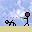
\includegraphics{../data/skills/Img/destreza.png}
It is how skillful, agile, flexible, among others similar adjectives, the creature is. An organism with much dexterity is able to do jugglings with knives and deviate easily from shots. A creature with low dexterity constantly stumbles at its legs and can't set a stone in the wall of a granary.\\
{\it Ameiva: Dexterity 8\\
Ratazana: Dexteterity 12\\
Ente: Dexterity 2}

\subsection{Constitution}

\includegraphics{../data/skills/Img/constituicao.png}
Measures how physical resistent is the organism. A creature with a lot of constitution is so resistent as a horse, able to injected venon on itself to withdrawn the antidote. A character with little constitution is constantly found in vegetative state, and, to him, the common influenza can be lethal.\\
{\it Ameiva: Constitution 12\\
Ratazana: Constitution 6\\
Ente: Constitution 26}

\subsection{Intelligence}

\includegraphics{../data/skills/Img/inteligencia.png}
Measures how smart or dumb the creature is. Organisms with a lot of intelligence can take 80 in OC2 (Computer Organization 2, more than 80 is only for Claudionor Disciples). Creatures too dumb only comunicate by gestures and grunts.\\
{\it Ameiva: Intelligence 6\\
Ratazana: Intelligence 2\\
Ente: Intelligence 16\\}

\subsection{Wisdow}

\includegraphics{../data/skills/Img/sabedoria.png}
Measures how much expert the creature is, knowing how to do in any life situations. An wisdow organism can make 10 years of post graduation without any problem. A creature with low wisdow can be lost in the way from the university restaurant to the bathroom.\\
{\it Ameiva: Wisdow 4\\
Ratazana: Wisdow 6\\
Ente: Wisdow 12}

\subsection{Charism}

\includegraphics{../data/skills/Img/carisma.png}
Measures how eloquent, imponent with words, inspirated or similar adjectives the creature is. A very charismatic organism can aglomerate students groups to invade the University Presidency Building. A not charismatic one can't make his dog obey him.\\
{\it Ameiva: Charism 25\\
Ratazana: Charism 6\\
Ente: Charism 8}

\subsection{Resistances}

\subsubsection{Fortitude}

\includegraphics{../data/skills/Img/fortitude.png}
Is the tested resistence when the creature is in contact with substances or feats that affect or can affect their physical integrity, altering some functions of their body, as poisons, coca-cola or effects of immediate death.

\subsubsection{Reflex}

\includegraphics{../data/skills/Img/reflexos.png}
Is the tested resistence when the creature is against instant effects that require quickly reactions to avoid physical damage.

\subsubsection{I Am Not A Fool}

\includegraphics{../data/skills/Img/vontade.png}
Is the resistence tested when the creature is against mental actions. With more {\it I am not a Foll}, more strong the creature is against compulsions incited by others or protected is its brain, to the point to immunize him of this kind of threat.

\subsection{Others}
DNT also use:

\subsubsection{Armature Class (AC)}

\includegraphics{../data/skills/Img/ca.png}
The Armature Class, or AC, measures how much the creature is external protected (like use of clothes, armors, defensives matrices) when receives some direct strike that affects its physical integrity. More AC means smaller chances of direct strike. The base AC is calculated by {\it 11+Armor+Dexterity Modifier+Varied Bonus}.

\subsubsection{Initiative}
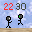
\includegraphics{../data/skills/Img/iniciativa.png}
Measures with how much velocity the creature reacts to threats in the battle begining. Hight bonus means that the chance to the creature make the first attack is greater.

\subsubsection{Life Points (LP)}

\includegraphics{../data/skills/Img/pv.png}
It's the vital resitance of the creature. Highter values, more strikes it can take before collapses. When the Life Points goes to zero, on common cases, the creature is unconscious in the ground. Values lesser than -10 means the creature is dead.

\subsubsection{Displacement}

\includegraphics{../data/skills/Img/deslocamento.png}
It's how much distance can the creature walk on some time interval. Is measured in meters.

\subsubsection{Extern Characters Things}
Are the visual details of the creature, like eye color, hair, size, sex and others.

\subsection{Levels}
Each class level works as 3 months of experience in the selected course class (or profession). The necessary number to evolute is the same as any D\&D like game.

\section{Playable Races}

\subsection{Strange Autistic}
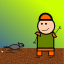
\includegraphics{../data/races/Img/autista.png}\\
{\it \" -Look at this boy! He is you when you were small!\\
 -No, Farrer, I was a normal and happy child..."\\
(Farrer to a Strange Autistic (Panda), Anamabeka's vocalist, when watching an Oblongs episode where one infant, with eyes of different sizes, sawed his bed utilizing a saw)\\}

Despite of, in the distance, looks like a common and normal person, this
tormented organism suffers serious psychological dysfunctions and
comportamentals detours. These creatures have the power to bring outside their
own world all the elements that exists there, sometimes confunding other races.
Feared by many and misunderstood by everybody, this organism is going to lead
their life as any other race, without put the others, or he, in risk.
Everybody has a little of Strange Autistic inside itself, be this autism a
world of wars and shots, fights and samurais, latin culture or styles of swords
and drums.

\subsubsection{Characteristics}
\begin{itemize}
\item{Being too much strange for someone else's eyes, the Strange Autistic receives -4 in all {\it social tests} when deal with an aim of opposite tendencies.}
\item{Understanding the fact that everybody is a little Strange Autistic, the Strange Autistic receives a bonus of + 2 in all {\it social tests} when deal with an aim of compatible tendencies.}
\item{The Strange Autistic possess, soon as in the first level, the feats {\it Only you are...} and {\it Confused Actions}}
\end{itemize}

\subsection{Boy / Paty}

\includegraphics{../data/races/Img/boy.png}\\
{\it "Ah friend, I can't, 'cause I'll do some biceps exercises today"\\
(Tico Bombadinho)\\}

Boys, and their female versions, Patys, are creatures endowed with a strange
fondness to body academies. Always wanting to be slenders to go to jet set
parties and rubbing with their oposite sex equivalents, they usually ignore
their friends of distinct races. But, by more upper they consider theirselves,
and despite they have a huge fondness themselves, this race is always the aim
of mockeries and jokes by other races.\\

\subsubsection{Characteristics}
\begin{itemize}
\item{Boys have {\it Driver} as class skill, since they are distinguished offenders of traffic laws.}
\item{Patys have +1 in {\it Diplomacy} since they always exhibit their bodies characteristics. For more horrendous than she was, she is able to "magically" alter herself in few hours.}
\item{By the aforesaid reasons, the Patys also receive + 2 in {\it Disguises}.}
\item{Boys and Patys receive +1 in {\it Constitution} due to the constant time they spend on body academies. If they no more go there, they'll lose this bonus and automatically become aim of jokes among others of their own race.}
\end{itemize}

\subsection{Gothic}

\includegraphics{../data/races/Img/gotico.png}\\
{\it "I have a problem..."
\\(Creepy Susie)}\\

With their nose facing the moon and their depressive way of life (that for them
are a bale), the Gothic live in groups since cemeteries up to Savassi plaza.
Always dressed entirely in black and with strange makeups, wandering by the
night reciting Álvares de Azevedo (Brazilian {\it Lord Byron} clone) and
claiming of their life to the other innocent races. 

They love the internet, but there they forget, from time to time, that they
hate the life, leaving visible flashes of joy and of that everything they do is
only pretend to other's eyes. 

\subsubsection{Characteristics}
\begin{itemize}
\item{\it Sun Weakness}
\item{\it Night Adoration}
\item{\it Laments of One Thousand Souls}
\item{Since Boys/Patys are hightly emotional, Gothics receive +2 in {\it Intimidate} against them.}
\end{itemize}

\subsection{Hippie}

\includegraphics{../data/races/Img/hippie.png}\\
{\it "They say that they want to save nature, but the only thing they do is smoke maryjane and smells bad!"\\ (Eric Cartman)}\\

Lovers of plants, animals, fungi, worms, air, wind, water, breeze, fire, heat,
in other words, everything that emanate something from nature and can transmit
them energy or karma (no, we aren't talking about Druid Elfs), the hippies can
be for hours listening to the wind voice or seeing little land worms entering
their bodies, since equiped with high LSD doses.\\

\subsubsection{Characteristics}
\begin{itemize}
\item{Since they have a lot of love for the nature, the el.., I've said, hippies, receive +5 in {\it Train Animals}.}
\item{Usually Hippies creatures aren't well accept by society, fearful of their subversives actions based on LSD, so, they receive -6 in {\it Free-pass}.}
\item{Hippies receive, in their first level, the feat {\it Lago Seco do Diabo (LSD)}.}
\end{itemize}

\subsection{Common Human}
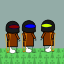
\includegraphics{../data/races/Img/humano.png}\\
{\it "Satana sum et nihil humanum a me alienum puto"\\
 (Demon talking to Ivan Karamazov)}\\

Also knowleged as {\it Homo Sapiens Sapiens}. An human is an human, uai! Look
the rest at your D\&D book cause I'm too busy to write normal things here. We
really hope that nobody owns the patent of the name "human" and we have to use
another denomination to this race in reason of copyright violations.

\subsubsection{Characteristics}
\begin{itemize}
\item{The Common Human is so normal and so common that don't own any extraordinary quality nor extraordinary defect.}
\end{itemize}

\subsection{Human Llama}

\includegraphics{../data/races/Img/llama.png}\\
{\it "Is he insane??"\\
("Oktober Fest"'s Queen, while looking at Farrer, the llama)}\\

Human llamas are humans that believe earnestly they are nearly descendants of
the Andes llamas. Usually they walk with a bolivian poncho, drink a lot of
water and think exactly like a llama.

\subsubsection{Characteristics}
\begin{itemize}
\item{\it Need Water}
\item{Human llamas receive +2 in {\it Intelligence}.}
\item{For having sociopats tendencies, the Human Llammas receive -4 in all {\it social tests}.}
\item{{\it I dislike you}}
\end{itemize}

\subsection{Headbanger}

\includegraphics{../data/races/Img/metaleiro.png}\\
{\it "Dark... "\\
(Anamatheus Iskurium)\\}

These creatures usually walk with black pants, black skirts (of bands or not)
and military boots. They wear this kind of clothes to "be different", althought
all of them use the same. They love to play all things they find thinking it
was a drum, and to sing the lyrics of the musics they love. Usually passed as
autistcs, these creatures walk with others headbangers (from 2 to 5) and have
the need to show others their "revolt". They are attracted easily by anything
that looks "malignant", for more rougher than it can be.

\subsubsection{Characteristics}
\begin{itemize}
\item{{\it Voluntary Autistim}}
\item{{\it Prompt Mosh}}
\item{Since Boys/Patys are hightly emotional, Headbangers receive +2 in {\it Intimidate} against them.}
\end{itemize}

\subsection{Skinhead Maniac}

\includegraphics{../data/races/Img/skin.png}\\
{\it \" - Is 'cause ther'are some peopl'in front of my house that puts a pagode in high volume on the weekends...\\
 - There is, so? Give me R\$500,00 and I'll five you a fragmentation granade to throw up there and end with their party!"\\
(Corrente, Skinhead Maniac, answering Gordo, Mechanical engineering frustrated studant)}\\

Skinhead Maniacs are a rare race in the campus. Without any comon sense, these
creatures don't lose time to finalize their objectives in the more directly
possible way. Walking alone in the world, they aren't capable to make friends
with any other race, always wanting to end those they dislike.

\subsubsection{Characteristics}
\begin{itemize}
\item{Skinhead Maniacs, since they have army's friends, can get any kind of heavy guns and walk freely with them. So, they receive the skill {\it Free-pass} for class skill for any choosed class.}
\item{{\it Insane Fury}}
\item{Since they don't have common sense, Skinhead Maniacs have to be of Alignment / Tendency {\it Capitalist Proprietary-Software} or {\it Chaotic Proprietary-Software}.}
\item{{\it Call Hordes}}
\item{Since they are solitary creatures, they can't walk in groups. Their unic reforce is the Hordes that goes away after the battle.}
\end{itemize}

\subsection{Mutant Human Cricket}
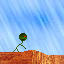
\includegraphics{../data/races/Img/grilo.png}\\
{\it "A tasty Cricket, please!"\\
(Logan in a barbecue restaurant)}\\

No one knows why, but mutant things started to habit Icex. With their diet
based on crickets or small hopping bugs, the Human Cricket have some
canibalistic habits and, for this, are not welcome by bugs. The habitat of the
Human Cricket is the famous Tyrol, near Barreiro, where they live happily
among their parents.

\subsubsection{Characteristics}
\begin{itemize}
\item{Since they eat Crickets, Human Crickts receive -4 in all {\it social tests} when threat with someone of their race or insects.}
\item{By obvious reasons, the Human Cricket receives +6 in {\it Jump}.}
\end{itemize}


\section{Alignment / Tendency}

The alignments and the tendencies in DccNiTghtmare are composed by the following possibilities\\

\subsection{Libertarian Free-Software Adept}
\includegraphics{../data/alignment/Img/libertarian.png} Libertarian Free-Software Adepts usually are creatures that believe in the free circulation of knowledge, without any intervention, be of governments, be of private groups or individuals. Usually they are adepts of public domain software.

\subsection{Center Free-Software Adept}
\includegraphics{../data/alignment/Img/gnu.png} Center Free-Software Adepts also believes in the free knowledge circulation, but, for them, the circulation hasn't to be as free as in public domain, but restrict to be free for all since continue free. Usually they are only adepts of GPL licences.

\subsection{Chaotic Free-Software Adept}
\includegraphics{../data/alignment/Img/beastie.png} Chaotic Free-Software are more permissive to the software license, since they are without charge and let full access to the source code.

\subsection{Functional Neutral} 
\includegraphics{../data/alignment/Img/canivete.png} Functional Neutral creatures don't have a solid position on software licenses. They are adepts of software that works correctly (and this concept is a lot vague).

\subsection{Center Neutral} 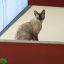
\includegraphics{../data/alignment/Img/muro.png} The thing more on top of the wall in the DccNiTghtmare's universe.  They have tendency to be favorable to what people near them are.

\subsection{Chaotic Neutral} 
\includegraphics{../data/alignment/Img/yang.png} Chaotic Neutral creatures sometimes are free software adepts, sometimes are proprietary software adepts, depending on their daily humor.

\subsection{Capitalist Proprietary-Software Adept}
\includegraphics{../data/alignment/Img/ruindows.png} Capitalist Proprietary-Software Adepts have in uncle Bill Portoe\$ their big idol. They want to be rich with the software they make, although, most of them, have their work explored by national software factories.

\subsection{Neutral Proprietary-Software Adept} 
\includegraphics{../data/alignment/Img/cifrao.png} Neutral Proprietary-Sorftware Adepts want to make money with their programs, but distrust of the absence of security on their Ruindow\$.

\subsection{Chaotic Proprietary-Software Adept}
\includegraphics{../data/alignment/Img/niquel.png} The wealth sometimes interest them, sometimes not, also uncle Portõe\$, although they consider the Free-Software Adepts as crazy guys.

\section{Classes}

\subsection{Administration Student}

\includegraphics{../data/classes/Img/administracao.png}
{\it "Steel with steel is bad..."\\(Zamboy, future Administration Student)}\\

Also knowledged as Taylor's  little boys, Administration Students are frequently found in self-help shelves of commercial bookstores. They enter in this course  since they not really know what want to their lifes (exacts science, human science, group  dynamics??) and, although in most of the cases don't possess NOTHING to administer, they think, vehemently, that are doing the helpful and certain thing to their lives.\\ 

{\bf Life Dice:} {\it d4}

\subsubsection{Attributes}
\begin{itemize}
\item{-2 {\it Intelligence}: Administration Students, definitively,  aren't know by their intelectual {\it (Am I wrong Elis Regina???)}.}
\item{-4 {\it Charism}: Charismatics??? Nor a little. A really dumb ass to find some of them in group.}
\item{+2 {\it Constitution}: The Taylor's Knowledges are a common part of the Administration Students, so their {\it Taylor's Bovinice} is always inerent.}
\end{itemize}


\subsubsection{Characteristics}
\begin{itemize}
\item{Since they are Taylor's fiel disciples, they receive +4 in {\it Taylor's Bovinice Skill}, also +4 em {\it Bizarre Clothes}, because in their dogmatic cult to Taylor they found bizarre things (and with maximun financial efficiency) to be their "clothes".}
\item{Everyone knows that the Administration Students have a lot of difficulty in assimilate other's opinions, and also to ask in a concise way some question, so they receive -6 in {\it Listen}.}
\end{itemize}

\subsubsection{Class Skills}
\begin{itemize}
{\it
\item{Appraise}
\item{Bizarrer Clothes}
\item{Bribe}
\item{Burglarize}
\item{Counterfeit}
\item{Foot-On-Man's-Genitals}
\item{Knowledge(administrative)}
\item{Professional Speech}
\item{Taylor's Bovinice}
}
\end{itemize}

\subsubsection{Skill Points}
{\bf Level 1}: (2 - Intelligence Modifier)x3\\
{\bf Other Levels}: 2 - Intelligence Modifier\\

\subsubsection{Special Feats}

\begin{center} \begin{tabular}{|c||c|c|c|}
\hline
{\bf Level}&{\bf Base Attack Bonus}&{\bf Fort./Refl./INF}&{\bf Feat}\\
\hline
1&+0&+0/+2/+2&{\it Esthetic Shock I}\\
\hline
2&+1&+1/+3/+3&\\
\hline
3&+1&+1/+3/+3&{\it Stun Attack}\\
\hline
4&+2&+2/+4/+4&\\
\hline
5&+2&+2/+4/+4&{\it Esthetic Shock II}\\
\hline
6&+3&+3/+5/+5&\\
\hline
7&+3&+3/+5/+5&{\it Improved Stun Attack}\\
\hline
8&+4&+4/+6/+6&\\
\hline
9&+4&+4/+6/+6&\\
\hline
10&+5&+5/+7/+7&{\it Web-Design}\\
\hline
11&+5&+5/+7/+7&\\
\hline
12&+6/+1&+6/+8/+8&\\
\hline
13&+6/+1&+6/+8/+8&\\
\hline
14&+7/+2&+7/+9/+9&\\
\hline
15&+7/+2&+7/+9/+9&{\it Esthetic Shock III }\\
\hline
16&+8/+3&+8/+10/+10&\\
\hline
17&+8/+3&+8/+10/+10&\\
\hline
18&+9/+4&+9/+11/+11&\\
\hline
19&+9/+4&+9/+11/+11&\\
\hline
20&+15/+10/+5&+16/+6/+7&{\it Supreme Esthetic Shock}\\
&&&{\it Aberration}\\
\hline
\end{tabular} \end{center}

{\it *INF = I'm not a Fool}\\

The previous table is a Base Bonus one, so they are without the {\it feats variations and race/class modifiers}.\\

\subsection{Biology Student}
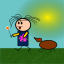
\includegraphics{../data/classes/Img/biologia.png}
{\it "This place is filled with arthropodes!"\\(Bin, that time, a Biology Student)}\\

Able to be for two weeks isoleted in the mountains making their "Field Works",
ambushing and observing the incredible and exciting ameiva's feed habits (and,
for it, sometimes mistaken as {\it Hippies} in their search for Feed-Karma),
the Biology Students are from all things a little: a little medicians, a little
hippies, a little computers, a little hot-dog sellers...\\

{\bf Live Dice:} {\it d8}

\subsubsection{Attributes}
\begin{itemize}
\item{+2 in {\it Dexterity}, since they always observe and follow in distinct terrains the ameivas (and also to open its body, counting how many worms it has)}
\item{-1 in {\it Strenght}, since their muscles atrophy after spent 12 hours inert observing the ameiva's coupling rituals.}
\end{itemize}

\subsubsection{Characteristics}
\begin{itemize}
\item{Since they are mistaken as {\it hippies}, Biology Students receive +6 in {\it Disguises} when disguised as hippie (and when not of this race), and -4 in {\it free-pass}, for the same reason (and also, when not of this race).}
\item{For the hard work observing ameivas, the Biology Student receveis +2 in {furtivity}}
\end{itemize}

\subsubsection{Class Skills}
\begin{itemize}
{\it 
\item{Disguises}
\item{Furtive}
\item{Hide}
\item{Knowledge (Biology)}
\item{Listen}
\item{Medical Loud Mouth}
\item{Observate}
\item{Out Of Time}
\item{Professional Speech}
\item{Scale}
\item{Train Animals}
}
\end{itemize}

\subsubsection{Skill Points}
{\bf Level 1}: (5 + Intelligence Modifier)x3\\
{\bf Other Levels}: 2 + Intelligence Modifier\\

\subsubsection{Special Feats}

\begin{center} \begin{tabular}{|c||c|c|c|}
\hline
{\bf Nível}&{\bf Base Attack Bonus}&{\bf Fort./Ref./INF}&{\bf Feat}\\
\hline
1&+0&+1/+2/+1&{\it Ameivas Adoration}\\
\hline
2&+1&+2/+3/+2&\\
\hline
3&+1&+2/+4/+3&\\
\hline
4&+2&+4/+5/+4&{\it Ameivas Worms}\\
\hline
5&+2&+4/+6/+5&{\it }\\
\hline
6&+3&+5/+7/+6&\\
\hline
7&+3&+5/+7/+6&{\it Arc Impulse}\\
\hline
8&+4&+6/+8/+7&\\
\hline
9&+4&+7/+9/+8&\\
\hline
10&+5&+7/+10/+8&{\it Mass Arthropods Attack}\\
\hline
11&+5&+8/+11/+9&\\
\hline
12&+6/+1&+8/+11/+9&\\
\hline
13&+6/+1&+9/+12/+10&\\
\hline
14&+7/+2&+10/+13/+11&\\
\hline
15&+7/+2&+11/+14/+12&{\it Darwin }\\
\hline
16&+8/+3&+12/+15/+13&\\
\hline
17&+8/+3&+13/+16/+14&\\
\hline
18&+9/+4&+14/+17/+15&{\it Stranglers Entes}\\
\hline
19&+9/+4&+14/+17/+15&\\
\hline
20&+13/+8/+3&+15/+18/+16&{\it Pleine Commande De Nature }\\
\hline
\end{tabular} \end{center}

The previous table is a Base Bonus one, so they are without the {\it feats variations and race/class modifiers}.\\

\subsection{Computer Science Student}

\includegraphics{../data/classes/Img/dcc.png}
{\it 
\"-I really don't know why I'm making this graduation...\\
- How not?? For the womans, obvious!"\\
(Gushm, Computer Science Student, answering the CS dilema)}\\

Computes Science Student is the most bizarre class in DccNiTghtmare (and,
paradoxically, the most common). They are know by their suicidal choices (the
first one is the graduation they choosed), their little patience to view what
their masters denominate "classes", the infinity time spent in Pratical
Exercises (TP) and the hate when they percept that it works perfectly, but their
masters won't look and appraise it, since CS teachers are displicents and
without any compromise with the graduation.\\

{\bf Live Dice:} {\it d8}

\subsubsection{Attributes}
\begin{itemize}
\item{+2 {\it Wisdow}: since all they are auto-teachers, because they can't count with theirs teachers.}
\item{-1 {\it Charism}: by their natural tendency to be qualified as Nerd, being one or not.}
\end{itemize}

\subsubsection{Characteristics}
\begin{itemize}
\item{Computer Science Students receive +5 in {\it fortitute} by support the hoax and boring that are their course and -2 in {\it reflexes} for a lot of time they spent in front of the computer.}
\end{itemize}

\subsubsection{Class Skills}
\begin{itemize}
{\it
\item{Drinking}
\item{Bluff}
\item{Knowledge (tecnology)}
\item{Knowledge: Suffer}
\item{Professional Speech}
\item{Hide}
\item{Listen}
\item{Operate Eletronic Objects}
\item{Prestidigitation}
\item{Out of Time}
}
\end{itemize}

\subsubsection{Skill Points}
{\bf Level 1}: (4 + Intelligence Modifier)x3\\
{\bf Other Levels}: 4 + Intelligence Modifier\\

\subsubsection{Special Feats}

\begin{center} \begin{tabular}{|c||c|c|c|}
\hline
{\bf Nível}&{\bf Base Attack Bonus}&{\bf Fort./Refl./INF}&{\bf Feat}\\
\hline
1&+0&+2/+0/+1&{\it Suicidal Choices}\\
\hline
2&+1&+3/+1/+2&\\
\hline
3&+2&+4/+2/+3&{\it Suffer Resistance}\\
&&&{\it Destroy Proprietary or Free Software}\\
&&&{\it addepts (tend)}\\
\hline
4&+3&+5/+3/+4&\\
\hline
5&+4&+6/+4/+5&{\it I Know and You don't}\\
\hline
6&+5&+7/+5/+6&\\
\hline
7&+5&+7/+5/+6&{}\\
\hline
8&+6/+1&+8/+6/+7&\\
\hline
9&+7/+2&+9/+7/+8&{\it World Conception}\\
&&&{\it Cybernetic Body}\\
\hline
10&+8/+3&+10/+7/+8&{\it OC2 Trauma}\\
\hline
11&+9/+4&+11/+8/+9&\\
\hline
12&+9/+4/+1&+11/+8/+9&{\it Improved Suffer Resistence}\\
\hline
13&+10/+5&+12/+9/+10&\\
\hline
14&+11/+6/+1&+13/+10/+11&\\
\hline
15&+12/+7/+2&+14/+11/+12&{\it Paralel Reality}\\
\hline
16&+13/+8/+3&+15/+12/+13&\\
\hline
17&+14/+9/+4&+16/+13/+14&\\
\hline
18&+15/+10/+5&+17/+14/+15&\\
\hline
19&+15/+10/+5&+17/+14/+15&\\
\hline
20&+16/+11/+6/+1&+18/+15/+16&{\it Chaos Matrix}\\
\hline
\end{tabular} \end{center}

The previous table is a Base Bonus one, so they are without the {\it feats variations and race/class modifiers}.\\

\subsection{Law Student}

\includegraphics{../data/classes/Img/direito.png}
{\it \" - Are we going to the bar taking one?\\
        - Yes, from whose?"\\(Typical dialog between two law students)}\\

Living at the Campus disguised as penguins, the Law Students are organisms
that, when perceive the minor possibility to make profits by some situation
they judge "juridic", will use of all their verborragy, deturpations and
sofisms to make it. Is always important to have a Law Student in your group
(party), be for avoiding other Law Students knowledge (and policial aparate) to
take advantages from you, or for taking advantages from others and avoid that
iminent punition.\\

{\bf Live Dice:} {\it d6}

\subsubsection{Attributes}
\begin{itemize}
\item{-2 {\it Intelligence}: For usually being stupids among anything that is not related with money;}
\item{-1 {\it Charism}: For their hungry will to take the last copeck of their victims;}
\item{+2 {\it Wisdow}: By can modify any situation to make money from it.}
\end{itemize}

\subsubsection{Characteristics}

\begin{itemize}
\item{Since they know anything about money, the Law Student receives +1 in {\it Appraise} on their first level.}
\end{itemize}

\subsubsection{Class Skills}
\begin{itemize}
{\it
\item{Art of the Escape}
\item{Appraise}
\item{Bluff}
\item{Conterfeit}
\item{Diplomacy}
\item{Foot on man's genitals}
\item{Free Pass}
\item{Get Information}
\item{Intimidate}
\item{Knowledge(law)}
\item{Knowledge: Suffer}
\item{Prestidigitation}
\item{Profissional Speech}
}
\end{itemize}

\subsubsection{Skill Points}
{\bf Level 1}: (6+Wisdow Modificator)x4\\
{\bf Other Levels}: 6+Wisdow Modification\\

\subsubsection{Special Feats}

\begin{center} \begin{tabular}{|c||c|c|c|}
\hline
{\bf Level}&{\bf Base Attack Bonus}&{\bf Fort./Ref./INF}&{\bf Feat}\\
\hline
1&+0&+0/+2/+0&{\it Lawyer Apprentice}\\
\hline
2&+1&+0/+3/+0&{\it - }\\
\hline
3&+2&+1/+3/+1&{\it Appraise +2}\\
\hline
4&+3&+1/+4/+1&{\it I am Wrong}\\
\hline
5&+3&+1/+4/+1&{\it }\\
\hline
6&+4&+2/+5/+2&{\it Appraise +3}\\
\hline
7&+5&+2/+5/+2&{\it }\\
\hline
8&+6/+1&+2/+6/+2&{\it - }\\
\hline
9 & +6/+1& +3/+6/+3 & {\it Appraise +4}\\
\hline
10 & +7/+2 & +3/+7/+3 & {\it -}\\
\hline
11 & +8/+3 & +3/+7/+3 & {\it }\\
\hline
12 & +9/+4 & +4/+8/+4 & {\it Appraise +5}\\
\hline
13 & +9/+4 & +4/+8/+4 & {\it Supreme Bluff}\\
\hline
14 & +10/+5 & +4/+9/+4 & {\it }\\
\hline
15 & +11/+6/+1 & +5/+9/+5 & {\it Appraise +6}\\
\hline
16 & +12/+7/+2 & +5/+10/+5 & {\it -}\\
\hline
17 & +12/+7/+2 & +5/+10/+5 & {\it }\\
\hline
18 & +13/+8/+3 & +5/+11/+5 & {\it Appraise +7}\\
\hline
19 & +14/+9/+4 & +6/+11/+5 & {\it }\\
\hline
20 & +15/+10/+5 & +6/+12/+6 & {\it Final Judgment}\\
\hline
\end{tabular} \end{center}

The previous table is a Base Bonus one, so they are without the {\it feats variations and race/class modifiers}.\\

\subsection{Physical Education Student}
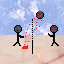
\includegraphics{../data/classes/Img/edfisica.png}
{\it "No!!! The swimming class is too complex!"\\(Typical Physical Education Student thought)}\\

Usually having "Soccer" and "Basketball" as classes, the dedicated (in the physical sense of the word) Students of Physical Education are things that value the muscular force above all.  With too muscles in the brain, those Students possess nothing less than a supernatural resistance in the head - in change of some points of Intelligence, really.  Finally, these boys are stars in the soccer but aren't distinguished students of mathematics (hardly knowing the fundaments of numbers).\\

{\bf Life Dice:} {\it d12}

\subsubsection{Attributes}
\begin{itemize}
\item{+3 {\it Strength}, due to the lot of hours kicking a ball.}
\item{+2 {\it Dexterity}, due to the hours fluctuating in the water.}
\item{+4 {\it Constituition}, for hours running in circles.}
\item{-6 {\it Intelligence} and {\it Wisdow}, since they abandoned the books in a remote past.}
\end{itemize}

\subsubsection{Characteristics}
\begin{itemize}
\item{The   Student   of   Physical   Education receives  +4  in  {\it Jump,   Scale,   Mount, Swimming,  Soccer,  Basketball},  finally, sports  in  general  or   anything that emanates physical power. They receive -5 in all {\it knowledges} by the simple fact of they have no idea of the meaning of this word, -4 in {\it Hide}, since they are coarse hulks, -2 in {\it listen}, therefore  the muscles take all ear's openings, also receive +1 of Natural Armor, +2 of {\it I Am Not A Fool} by the fact of their brain stop function sometimes.}
\item{The  Student  receives  -4 in {\it Train Animals}, since, by haven't absolute control of their muscles,  there  is  a chance of crushing the animal; -3 in {\it Direction} cause they usually get lost among their own muscles. Also  they possess -2 in {\it Bluff}, therefore their muscles practically possess own life and easily contratic them in their lies.}
\item{By  the  corpulent size of their muscles and the total absence of control, the Student of Physical Education have 60\% of chance to tumble in battle.}
\item{Beyond this, the Student of Physical Education can't buy points in skills whose ability key is Intelligence.}
\item{Since extremely limited on its skills, the Physical Education Student don't have any limit on {\it Sports} graduation.}
\end{itemize}

\subsubsection{Class Skills}
\begin{itemize}
{\it 
\item{Bascketball}
\item{Jump}
\item{Soccer}
\item{Swimming}
\item{Volley}
\item{So, only one: sports.}
}
\end{itemize}

\subsubsection{Skill Points}
{\bf Level 1}: (9+Intelligence Modifier)x3\\
{\bf Other Levels}: 9+Intelligence Modifier\\

\subsubsection{Special Feats}

\begin{center} \begin{tabular}{|c||c|c|c|}
\hline
{\bf Level}&{\bf Base Attack Bonus}&{\bf Fort./Ref./INF}&{\bf Feat}\\
\hline
1&+1&+5/+0/+2&{\it Improvise Weapons (Balls)}\\
\hline
2&+2&+6/+1/+3&\\
\hline
3&+3&+6/+2/+4&{\it Shrink Items}\\
\hline
4&+4&+7/+3/+4&\\
\hline
5&+5&+7/+4/+5&\\
\hline
6&+6/+1&+8/+5/+6&\\
\hline
7&+7/+2&+9/+5/+6&{\it Virtually Undestructible}\\
\hline
8&+8/+3&+10/+6/+7&\\
\hline
9&+9/+4&+11/+7/+8&\\
\hline
10&+10/+5&+12/+7/+8&{\it I am Strong!}\\
\hline
11&+11/+6/+1&+13/+8/+9&\\
\hline
12&+12/+7/+2&+14/+8/+9&\\
\hline
13&+13/+8/+3&+15/+14/+10&{\it Improvise Weapons Improved}\\
\hline
14&+14/+9/+4&+15/+10/+11&\\
\hline
15&+15/+10/+5&+16/+10/+12&{\it Powerful Esophagus}\\
\hline
16&+16/+11/+6/+1&+17/+11/+13&\\
\hline
17&+17/+12/+7/+2&+18/+11/+13&\\
\hline
18&+18/+13/+8/+3&+19/+12/+14&\\
\hline
19&+19/+14/+9/+4&+20/+12/+14&\\
\hline
20&+30/+25/+20/+15/+10/+5&+30/+4/+10&{\it Abominable Mutation}\\
\hline
\end{tabular} \end{center}

The previous table is a Base Bonus one, so they are without the {\it feats variations and race/class modifiers}.\\

\subsection{Journalism Student}
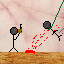
\includegraphics{../data/classes/Img/jornalismo.png}
{\it "The judge thinks he is God, the Medic plays God. The journalist, if he isn't God, convinces you that he is" (Matheus de Paula, Journalism student)}\\

Graduating in the arts of deceit a cheating, the journalism student is a writing master. With words, he can create events, stun his enemies, swindle his audience towards other habilities.\\
Despite of being college friends, these malicious organisms can be very rude to each other, not being common to see them in large groups. But they can easily join the masses, to gather as much information as possible.\\

{\bf Life Dice}: d6


\subsubsection{Attributes}
\begin{itemize}
\item{-2 Strenght - as they are usually deep involved in mental work, these organisms don't find time or will to exercise their muscles}
\item{+2 Intelligence - Journalism students have a "know it all" need, increasing their intelligence}
\item{+1 Charisma - Despite of being extemely hard criticals, these organisms can dissimulate their true nature, being very kind to their audience and information sources.}
\end{itemize}

\subsubsection{Characteristics}

\begin{itemize}
\item{Impartiality - Before choosing this class, the Journalism student rolls a d100. If the result is between 1 and 99, he can't be neutral. Else, he can be a Journalism Student with any alingment.}
\item{Journalism students neglects any penalties to their social tests, for being able to survive in turbulent environments.}
\item{As long as the Journalism Student speaks the targets language, he will never be ignored.}
\end{itemize}

\subsubsection{Class Skills}
\begin{itemize}
   \item{Appraise}
   \item{Bluff}
   \item{Diplomacy}
   \item{Disguises}
   \item{Foot-On-Man-Genitals}
   \item{Free-Pass}
   \item{Furtive}
   \item{Get Informations}
   \item{Hide}
   \item{Intimidate}
   \item{Knowledge(All)}
   \item{Listen}
   \item{Observate}
   \item{Professional Speech}
   \item{Speak Idiom}
\end{itemize}

\subsubsection{Skill Points}
{\bf Level 1}: (5+Intelligence Modifier)x3\\
{\bf Other Levels}: 5+Inteligence Modifier\\

\subsubsection{Special Feats}

\begin{center} \begin{tabular}{|c||c|c|c|}
\hline
{\bf Nível}&{\bf Bônus Base Ataque}&{\bf Fort./Refl./NSB}&{\bf Habilidade}\\
\hline
1&+0&+0/+1/+3&{\it Contacts}\\
\hline
2&+1&+0/+2/+4&{\it Aditional Language}\\
\hline
3&+2&+1/+2/+5&{\it Incisive Critic}\\
\hline
4&+3&+1/+3/+5&\\
\hline
5&+4&+2/+4/+5&\\
\hline
6&+4&+3/+5/+6&{\it Wasn't That What I've Said}\\
\hline
7&+5&+3/+5/+7&\\
\hline
8&+5&+3/+5/+8&\\
\hline
9&+6/+1&+3/+6/+9&\\
\hline
10&+7/+2&+4/+6/+10&{\it Devil Tongues}\\
\hline
11&+8/+3&+4/+7/+11&{\it Sarcastic Critic}\\
\hline
12&+8/+3&+4/+8/+12&\\
\hline
13&+9/+4/+1&+5/+9/+13&{\it Aditional Language}\\
\hline
14&+9/+4&+6/+10/+14&\\
\hline
15&+10/+5&+7/+11/+15&\\
\hline
16&+11/+6/+1&+8/+12/+16&{\it Serpent Tongue}\\
\hline
17&+11/+6/+1&+8/+12/+17&\\
\hline
18&+12/+7/+2&+9/+13/+18&\\
\hline
19&+12/+7/+2&+9/+13/+19&{\it Know Everything}\\
\hline
20&+13/+8/+3&+10/+13/+20&{\it Shameful Critic}\\
\hline
\end{tabular} \end{center}

\subsection{Mechanical Engineering Student}

\includegraphics{../data/classes/Img/engmecanica.png}
{\it "Today we'll see the comprex prane pracle probrem!"\\ (Haroldão, Mechanical teacher)}\\

The student of mechanical engineering is the campus most frustrated person. After enter the faculty in the hope of learn everything about cars, planes, boats and other mechanical structures of high complexity, they uncover that the world is summarized to {\it F = m*a}. In the possession of that simple equation and of absurd quantities of inexplicable calculations, the teachers of physics make their life a hell in the basic course. In the specific classes they realize that the world was happy in the basic cycle. Generally they're seen in all classes inside the Exacts Institute, therefore no one of is going to finish the course regularly.

{\bf Life Dice: } {\it d8}

\subsubsection{Attributes}
\begin{itemize}
\item{+3 {\it Intelligence}: Students  of Mechanics are going to study crazy, if they want to  do something more than  hold tight bolts in their lifes.}
\item{+2 {\it Wisdow}: Due  to the quantity of information about steels,  kinds  of   tempera,   tools  of plants,  electronic   systems  and  other things that  are  obliged to swallow.}
\item{-2 {\it Strength}: One  time that the  mouse  for  design  in  AutoCAD doesn't weigh much.}
\end{itemize}


\subsubsection{Characteristics}
\begin{itemize}
\item{A  student  of Mechanics always suffers a penalty of  -10  in  any  kind  of  tests against things of female sex.  The  total absence  of  contact  with  that  kind of agency causes a  barely unruly  frenzy in the  student,  that  should  do a test of I Am Not A Fool (with the penalty of -10) to not jump wildily on top of the female. In the  case  of fail, the student enters in  frenzy  and  will  try  with  all his forces to "copulate" with the same one.}
\end{itemize}

\subsubsection{Class Skills}
\begin{itemize}
\item{Conduction}
\item{Drinking}
\item{Knowledge(material)}
\item{Operate Eletronic Objects}
\item{Operate Mechanical Objects}
\item{Observate}
\item{Professional Speech}
\end{itemize}

\subsubsection{Skill Points}
{\bf Level 1}: (6+Intelligence Modifier)x3\\
{\bf Other Levels}: 6+Inteligence Modifier\\

\subsubsection{Special Feats}
\begin{center} \begin{tabular}{|c||c|c|c|}
\hline
{\bf Level}&{\bf Base Attack Bonus}&{\bf Fort./Ref./INF}&{\bf Feat}\\
\hline
1&+0&0/1/0&{\it Criate Objects }\\
\hline
2&+1&1/2/1&{\it Skill Focus:}\\
 & & & {\it Operarate Mechanic Object}\\
\hline
3&+1&1/2/1&\\
\hline
4&+2&2/3/2&{\it Improved Criate Objects}\\
\hline
5&+2&2/3/2&{\it Improved Skill Focus:}\\
&&&{\it Operate Mechanic Object}\\
\hline
6&+3&+3/+4/+3&\\
\hline
7&+3&+3/+4/+3&\\
\hline
8&+4&+4/+5/+4&{\it The Inertia Principle}\\
\hline
9&+4&+4/+5/+4&\\
\hline
10&+5&+5/+6/+5&\\
\hline
11&+5&+5/+6/+5&{\it Battle Construct}\\
\hline
12&+6/+1&+6/+7/+6&\\
\hline
13&+6/+1&+6/+7/+6&\\
\hline
14&+7/+2&+7/+8/+7&{\it Action and Reaction}\\
\hline
15&+7/+2&+7/+8/+7&\\
\hline
16&+8/+3&+8/+9/+8&\\
\hline
17&+8/+3&+8/+9/+8&{\it Like a child on Slide}\\
\hline
18&+9/+4&+9/+10/+9&\\
\hline
19&+9/+4&+9/+10/+9&\\
\hline
20&+10/+5&+10/+11/+10&{\it F = m * a}\\
\hline
\end{tabular} \end{center}

The previous table is a Base Bonus one, so they are without the {\it feats variations and race/class modifiers}.\\

\subsection{Medicine Student}

\includegraphics{../data/classes/Img/medicina.png}
{\it "If  I've  tried  Physiotherapy  there, I should passed  in first place with the points I've made in Medicine."\\
(Mattar, Medician  Student  answering the provocation   of  Wanúcia,  Physiotherapy Student)}\\

The Medicine Student is the thing that abdicated to their social life in change of an anormal dedication to study, believing they'll be something in life. Those things haven't any cleverness, one time they base their lifes in theories and more theories. To be of this class, the character need to be submitted to any hideous attitude, like drown hookies, public peversion, among others that result in death.\\

{\bf Life Dice:} {\it d6}.

\subsubsection{Atributtes}
\begin{itemize}
\item{+1 {\it Strenght}: although  being  theory  creatures,  they usually  spent  their  money  in physical academies.}
\item{+2 {\it Intelligence}: by  their  dedication  to  the  study.}
\item{-4 {\it Wisdow}: since their attention is only for the books, these  creatures  haven't any cleverness.}
\end{itemize}

\subsubsection{Characteristics}
\begin{itemize}
\item{Frequently in the studies, the Medicine Student forgot to grow up, being very susceptible to questions, receiving -3 in all {\it I am not a Fool} (these modifier fall to -6 when the target is their father  or mother)}
\item{Those creatures recive  +4 in  all  {\it Bluff} tests, one time that all bluff they made, for more ridiculous they are, can  really (and easily) be true.}
\item{They Receive +2 in {\it diplomacy} when talking to boys and patys and -2 when talking to other race.}
\item{They receive -4 in {\it diplomacy} when talking to Physiotherapy Students.}
\end{itemize}

\subsubsection{Class Skills}
\begin{itemize}
{\it
\item{Bohemia}
\item{Bribe}
\item{Conduction}
\item{Heal}
\item{Intimidate}
\item{Knowledge(medicine)}
\item{Knowledge: Suffer}
\item{Medical Loud Mouth}
\item{Out of Time}
\item{Professional Speech}
}
\end{itemize}

\subsubsection{Skill Points}
{\bf Nível 1}: (2+Modificador de Inteligência)x3\\
{\bf Níveis subsequentes}: 2+Modificador de Inteligência\\

\subsubsection{Special Feats}

\begin{center} \begin{tabular}{|c||c|c|c|}
\hline
{\bf Level}&{\bf Base Attack Bonus}&{\bf Fort./Ref./INF}&{\bf Feat}\\
\hline
1&+0&+1/+0/+2&{\it Exothic Weapon (bistoury)}\\
&&&{\it Knowledge Skills}\\
&&&{\it Hipocrates Oath}\\
\hline
2&+1&+2/+1/+3&{\it Rake}\\
\hline
3&+2&+3/+1/+4&\\
\hline
4&+3&+3/+2/+4&{\it Placed Blow}\\
\hline
5&+4&+4/+2/+5&{\it Dona Nobis Pacem}\\
&&&{\it Heal Wounds}\\
\hline
6&+5&+5/+3/+5&\\
\hline
7&+5&+6/+4/+6&{\it Veins and Arteries}\\
\hline
8&+6/+1&+6/+5/+7&\\
\hline
9&+7/+2&+6/+6/+8&{\it Heal Diseases}\\
\hline
10&+8/+3&+7/+7/+9&{\it I am Strong!}\\
&&&{\it I am Study!}\\
&&&{\it I am Slow!}\\
\hline
11&+9/+4&+8/+8/+10&\\
\hline
12&+10/+5&+8/+8/+11&\\
\hline
13&+11/+6/+1&+9/+8/+12&\\
\hline
14&+12/+7/+2&+10/+9/+13&{\it Body Knowledge}\\
\hline
15&+12/+7/+2&+10/+9/+14&\\
\hline
16&+13/+8/+3&+11/+9/+15&{\it Improved Body Knowledge}\\
\hline
17&+13/+8/+3&+11/+10/+15&\\
\hline
18&+14/+9/+4&+12/+10/+16&\\
\hline
19&+14/+9/+4&+12/+10/+16&\\
\hline
20&+15/+10/+5&+26/+4/+10&{\it Tu Fui, Ego Eris}\\
\hline
\end{tabular} \end{center}

The previous table is a Base Bonus one, so they are without the {\it feats variations and race/class modifiers}.\\

\subsection{Music Student}

\includegraphics{../data/classes/Img/musica.png}
{\it "Without you I sound nothing."\\
     (Typical commentary of a Lyric-man to a Musician - in Portuguese, sounds like: "Without you I am Nothing")}\\

In  a  scientific   world,   few   people adventure in a different  concept, follow some art source, like  music.  The  Music Student  is  a  creature   with   extreme patience to learn all tecnics related  to ternary  compass  atonalisms,  have   the capacity to realize them and  a distorced like to play one of the most bizarre  and ocult musical instrument. \\

{\it Note of the Creator: "Based  on  the idea that musical likes are distints  and only the the most understood  ones  appreciate distinct rhythms (obviously all ones that aren't  atempts  to   kill,  for bad, the musical theory), the class was made.  So, the same sound, Bach for example, can  be a beautifull music or  something  boring, depending  from  the  ear   who   listen. Probably a progressive fan will like Bach but a fan of Tati-Quebra-Barraco, without any musical sense, will think  Bach=shit. So, the Music Student will be a  virtuous misunderstood.

{\bf Life Dice: }{\it d6}\\ 

\subsubsection{Atributtes}
\begin{itemize}
\item{-4 of {\it Strenght} by  the fact  that their muscles atrophy for aren't used more than the much needed to play their instrument;}
\item{-1 of {\it Constitution} for hours  spent  in a closed ambient, playing;}
\item{+2 of {\it Dexterity} for having the ability to play  a  Gb7M  or  a  Am\#5/7/9  on  their strange musical instrument;}
\item{+1 of {\it Intelligence} for  know those notes, how  they  are  created  and  all musical theory envolved on their creation;}
\item{+2 of {\it Charism} for  the  capacity  to joy people.}
\end{itemize}

\subsubsection{Characteristics}
\begin{itemize}
\item{Cause of the extense and hard work  since they were childs, the Music Student  have incredible   capacity   to   play   their bizarre  instrument,  receiving  the   +8 bonus when playing it.}
\item{The Music Student need to have  at  least one graduation on Play Instrument, on one presented  at   the    Bizarre    Musical Instruments List.}
\end{itemize}

{\bf Bizarre Musical Instruments List}:\\
\begin{itemize}
{\it 
\item{Bugle}
\item{Bassoon}
\item{Oboé}
\item{Trompete}
\item{Tube}
}
\end{itemize}

\subsubsection{Class Skills}
\begin{itemize}
{\it 
\item{Bizarre Clothes}
\item{Bohemia}
\item{Knowledge(music)}
\item{Listen}
\item{Performate}
\item{Play Instrument(Bizarre One)}
\item{Professional Speech}
}
\end{itemize}

\subsubsection{Skill Points}
{\bf First Level}: (3+Intelligence Modifier)x3\\
{\bf Other Levels}: 3+Intelligence Modifier\\

\subsubsection{Special Feats}

\begin{center} \begin{tabular}{|c||c|c|c|}
\hline
{\bf Level}&{\bf Base Attack Bonus}&{\bf Fort./Ref./INF}&{\bf Feat}\\
\hline
1&+0&+0/+0/+4&{\it Play Melody}\\
&&&{\it Melolody - Calm Music}\\
\hline
2&+1&+0/+0/+5&\\
\hline
3&+1&+1/+1/+6&{\it Melody - Happy Melody}\\
\hline
4&+1&+2/+2/+7&\\
\hline
5&+2&+2/+2/+8&{\it Melody - Battle Rythim}\\
\hline
6&+2&+3/+3/+9&\\
\hline
7&+2&+4/+4/+10&{\it The Hamelin Flutter}\\
\hline
8&+3&+4/+4/+11&\\
\hline
9&+3&+5/+5/+12&{\it Melody - Tranquility}\\
 & & & {\it Serenata}\\
\hline
10&+4&+5/+5/+12&\\
\hline
11&+4&+6/+6/+13&{\it Melody - Entertainer Chords}\\
\hline
12&+5&+6/+6/+14&\\
\hline
13&+5&+7/+7/+15&{\it The Hamelin Flutter -}\\
&&&{\it Children Concert}\\
\hline
14&+6/+1&+7/+7/+15&\\
\hline
15&+6/+1&+8/+8/+16&{\it Melody - Fortitude Chant}\\
\hline
16&+7/+2&+8/+8/+16&\\
\hline
17&+7/+2&+9/+9/+17&{\it Melodiy - Epic Chords}\\
\hline
18&+8/+3&+9/+9/+17&\\
\hline
19&+9/+4&+10/+10/+18&{\it The Hamelin Flutter -}\\
&&&{\it Forbidden Concert}\\
\hline
20&+10/+5&+11/+11/+19&{\it Melody - Perfect Harmony}\\
\hline
\end{tabular} \end{center}

The previous table is a Base Bonus one, so they are without the {\it feats variations and race/class modifiers}.\\

\subsection{Occupational Therapy Student}
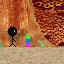
\includegraphics{../data/classes/Img/to.png}
{\it \" - Hey,  girls  from  OT, answer me  a question  I  have  since  enter  the university...\\
        - No,  We  also  don't  know to  what our faculty is made for and are bored  by the others asking us about it!"\\
        (Turmalina,  Computer  Science   Student, asking three OT Students)}\\

Usually   little    and    fragile,   the Occupational Therapy Students can be high emoted  watching  the  most  previsible mexican novel. Known by the "hard"  group therapies  they  call "Academic Classes", and for the hours spent painting a little paper like a three years child (and FOR a three   years    child),    calling    it "Scientific  Project",  the  OT  Students can't  explain  to  what  their course is (it's one  of  the  universe's  secrets), their  life  is,  their  clients,   their friends,   their   bass,  the  Anamabeka, their..., finally... but sure  know  what happened at the previous  chapter  of the midday television novel.

{\bf Life Dice:}{\it d4}\\

\subsubsection{Atributtes}
\begin{itemize}
\item{-2 {\it Intelligence}, for spent too much time watching TV novels.}
\item{+1 {\it Wisdow}, or the inutiles knowledges obtained watching TV novels.}
\item{+3 {\it Charism}, or  not  study  at   the Exacts Sciences Institute (ICEX), usually being pleasants.}
\end{itemize}


\subsubsection{Characteristics}
\begin{itemize}
\item{For usually have some rare  beauty to the ICEX, the OT Students receive +10 in  all social tests against Students  from  that Institute.}
\item{Receive -12 in {\it furtive} and {\it hide}, and +5 in {\it intimidadte} when in a radius of 30m of at least one ICEX Student.}
\item{OT Students have  the  tendency  to  play that  musical  instrument  someone  calls bass  (and  maybe  for  this,  forgot  by Anamabeka), receiving -4 in {\it observate}.}
\end{itemize}


\subsubsection{Class Skills}
\begin{itemize}
{\it
\item{Bluff}
\item{Bohemia}
\item{Diplomacy}
\item{Get Information}
\item{Medical Loud Mouth}
\item{Knowledge(theraphy)}
\item{Play Musical Instrument(Bass)}
\item{Professional Speech}
\item{See Lies}
}
\end{itemize}

\subsubsection{Skill Points}
{\bf First Level}: (5+Charism Modifier)x3\\
{\bf Other Levels}: (2+Charism Modifier)x2\\


\subsubsection{Special Feats}

\begin{center} \begin{tabular}{|c||c|c|c|}
\hline
{\bf Level}&{\bf Base Attack Bonus}&{\bf Fort./Ref./INF}&{\bf Feat}\\
\hline
1&+0&+0/+0/+2&{\it Group Therapy I}\\
\hline
2&+1&+0/+0/+2&\\
\hline
3&+1&+1/+1/+3&{\it Crocodile Tears}\\
\hline
4&+1&+2/+2/+3&\\
\hline
5&+2&+2/+2/+4&\\
\hline
6&+2&+3/+3/+4&{\it Group Therapy II}\\
\hline
7&+2&+3/+3/+5&\\
\hline
8&+3&+4/+4/+5&\\
\hline
9&+3&+4/+4/+6&\\
\hline
10&+4&+4/+4/+6&\\
\hline
11&+4&+5/+5/+7&\\
\hline
12&+5&+5/+5/+7&{\it Group Therapy III}\\
\hline
13&+5&+6/+6/+8&\\
\hline
14&+6/+1&+6/+6/+9&{\it Icex Shock}\\
\hline
15&+6/+1&+7/+7/+10&\\
\hline
16&+7/+2&+7/+7/+11&\\
\hline
17&+7/+2&+8/+8/+12&\\
\hline
18&+7/+2&+8/+8/+13&\\
\hline
19&+8/+3&+9/+9/+14&\\
\hline
20&+8/+3&+9/+9/+15&{\it Supreme Group Therapy}\\
\hline
\end{tabular} \end{center}

The previous table is a Base Bonus one, so they are without the {\it feats variations and race/class modifiers}.\\

\subsection{Philosophy Student}

\includegraphics{../data/classes/Img/filosofia.png}
{\it "Better die by vodka than by boredom"\\ (Vladmir Maiakovsky)}\\

Not satisfied with don't want nothing for their life, the Philosophy Student enter the university with just one objective: to perfect this wanting nothing.  Adepts  of drinking beer and of to do nothing, mixing their time between one and another  activity, the Philosophy Student become the bohemian master and full of hot air.\\

{\bf Life Dice:} {\it d6}

\subsubsection{Attibutes}
\begin{itemize}
\item{+2 {\it Constitution}: because their body is barely of a monk, fully usual to the alcohol.}
\item{-2 {\it Wisdow}: Since they only study complex things, the Philosophy  Student  easily  forgets  all pratical and common things of  the  life.}
\item{+2 {\it Charism}: For spending almost all their student's life in pubs, the  Philosophy  Student acquire some kind of aptitude to deal with others.}
\end{itemize}

\subsubsection{Characteristics}
\begin{itemize}
\item{The Philosophy Student receive +4 in {\it Knowledge(classic)} for the few they study at the university.}
\item{Receive +4 in {\it Bohemia} cause they are always on Pubs}
\item{Receive -4 on all in all dexterity related tests one time they are frequently drunk.}
\item{For don't make any (or very few) classes, the Philosophy Student receive -4 in {\it Out of time.}.}
\end{itemize}

\subsubsection{Class Skills}
\begin{itemize}
{\it 
\item{Art of the Escape}
\item{Bluff}
\item{Bohemia}
\item{Drinking}
\item{Furtive}
\item{Hide}
\item{Knowledge(classic)}
\item{Professional Speech}
}
\end{itemize}

\subsubsection{Skill Points}
{\bf Level 1}: (7+Intelligence Modifier)x3\\
{\bf Other Levels}: 7+Intelligence Modifier\\

\subsubsection{Special Feats}

\begin{center} \begin{tabular}{|c||c|c|c|}
\hline
{\bf Level}&{\bf Base Attack Bonus}&{\bf Fort./Ref./INF}&{\bf Feat}\\
\hline
1&+0&+2/+0/+1&{\it Drunk Fight}\\
&&&{\it Turn, Turn, Turn!} \\
\hline
2&+1&+3/+1/+2&\\
\hline
3&+1&+4/+2/+3&{\it Additional Feat}\\
\hline
4&+1&+5/+3/+4&\\
\hline
5&+2&+6/+4/+5&{\it Temporary Glucose Addition}\\
\hline
6&+2&+7/+5/+6&\\
\hline
7&+3&+7/+5/+6&\\
\hline
8&+3&+8/+6/+7&{\it Additional Feat}\\
\hline
9&+4&+9/+7/+8&\\
\hline
10&+4&+10/+7/+8&{\it Improved Drunk Fight}\\
\hline
11&+5&+11/+8/+9&\\
\hline
12&+5&+11/+8/+9&{\it Iron Liver}\\
\hline
13&6/+1&+12/+9/+10&\\
\hline
14&+7/+2&+13/+10/+11&\\
\hline
15&+7/+2&+14/+11/+12&{\it Cirrhosis Cloud}\\
\hline
16&+8/+3&+15/+12/+13&\\
\hline
17&+8/+3&+16/+13/+14&{\it Additional Feat}\\
\hline
18&+9/+4&+17/+14/+15&\\
\hline
19&+9/+4&+17/+14/+15&\\
\hline
20&+10/+5&+18/+15/+16&{\it Supreme Drunk Fight}\\
\hline
\end{tabular} \end{center}

The previous table is a Base Bonus one, so they are without the {\it feats variations and race/class modifiers}.\\

\subsection{Physiotherapy Student}

\includegraphics{../data/classes/Img/fisioterapia.png}
{\it "You should have studied and entered the Federal University!"\\
     (Wanúcia, Pysiotherapy Student angry with Mattar, Medicine Student)}\\

Medicine Students arqui-rivals, the Physiotherapy Student feeds a mortal hate whith their half-blood brothers. The Physiotherapy Student, althought have something similar with the Medicine ones (like elves and half-elves), hate them with all their forces because the little medicians passed in the place that the physiotherapy one always want. The Physiotherapy Student usually works at physical academies, to better look for their victims.\\

{\bf Life Dice:} {\it d8}

\subsubsection{Atributtes}
\begin{itemize}
\item{+1 {\it Dexterity}: for hard study the humam body mobility, they can realize some achievements.}
\item{+1 {\it Intelligence}: all Physiotherapy Student los one or more years trying to be a Medicine Student.}
\item{-2 {\it Wisdow}: cause of the effort to be a Medicine Student, the little Physiotherapy inherit this penalty.}
\end{itemize}

\subsubsection{Characteristics:}
\begin{itemize}
\item{Feeding the hate for their medicine rivals, the Physiotherapy receive  ac class bonus agains't them, of +1 on all {\it attacks} agains't medicians.}
\item{They receive +3 on all {\it listen, observate, bluff} and {\it I am Not a Fool} tests when targeting Medicine Students}
\item{Because they are failed Medicians, any chance of social interaction when there are Medicine Students in a radius of 20m, the Physiotherapy Student will receive -5 in all {\it social skills}. If they fail in a test by 5 or more, they will commit suicide.}
\end{itemize}

\subsubsection{Class Skills}
\begin{itemize}
{\it 
\item{Disguises}
\item{Heal}
\item{Knowledge(medicine)}
\item{Medical Loud Mouth}
\item{Professional Speech}
}
\end{itemize}

\subsubsection{Skill Points}
{\bf First Level}: (3+Intelligence Modifier)x3\\
{\bf Other Levels}: 3+Intelligence Modifier\\

\subsubsection{Special Feats}

\begin{center} \begin{tabular}{|c||c|c|c|}
\hline
{\bf Level}&{\bf Base Attack Bonus}&{\bf Fort./Ref./INF}&{\bf Feat}\\
\hline
1&+0&+1/+2/+0&{\it Favorite Prey -}\\
&&&{\it Medicine Student}\\
\hline
2&+1&+1/+3/+1&{\it Rake}\\
\hline
3&+2&+2/+4/+2&\\
\hline
4&+3&+2/+5/+3&{\it Favorite Prey II -}\\
&&&{\it Medicine Student}\\
\hline
5&+4&+3/+6/+4&\\
\hline
6&+5&+3/+7/+5&\\
\hline
7&+5&+4/+8/+5&{\it Incapacitate Blow}\\
\hline
8&+6/+1&+4/+9/+5&\\
\hline
9&+7/+2&+5/+10/+6&\\
\hline
10&+8/+3&+6/+10/+6&{\it Favorite Prey III -}\\
&&&{\it Medicine Student}\\
\hline
11&+9/+4&+7/+12/+6&\\
\hline
12&+10/+5&+8/+13/+7&\\
\hline
13&+11/+6/+1&+9/+14/+8&{\it Professional Pride}\\
\hline
14&+12/+7/+2&+10/+15/+8&\\
\hline
15&+12/+7/+2&+10/+15/+8&{\it Fovorite Prey -}\\
&&&{\it Medicine Student}\\
\hline
16&+13/+8/+3&+12/+16/+8&{\it Error Indiction}\\
\hline
17&+13/+8/+3&+12/+16/+9&\\
\hline
18&+14/+9/+5&+13/+17/+9&\\
\hline
19&+14/+9/+5&+13/+17/+10&\\
\hline
20&+15/+10/+5&+14/+18/+10&{\it Favorite Prey -}\\
&&&{\it Medicine Student}\\
&&&{\it Prey Knowledge - }\\
&&&{\it Medicine Student}\\
\hline
\end{tabular} \end{center}

The previous table is a Base Bonus one, so they are without the {\it feats variations and race/class modifiers}.\\

\section{Feats}

\subsection{Race: Strange Autistic}

\subsubsection{Confused Actions}
{\bf Pre-requisite}: Strange Autistic\\
Cause they are entirely misunderstood, these organisms are capable to confuse his interlocutors with their actions. Having success in a test of {\it Bluff} against {\it I Am Not A Fool} of the aim, the Strange Autistic is going to leave the aim confused for 1d4 turns.

\subsubsection{Only You Are...}
 {\bf Pre-requisite}: Strange Autistic\\
Due to his strange/bizarre manner of act, the Strange Autistic is capable of amaze an aim, making it loses the turn action by be, of some forms, dumbfounded {\it (laughing, crying, looking strange, between other possible actions)}.  The Strange Autistic roll {\it 1d20 + character level/2} against the {\it I Am Not A Fool} of the aim.

\subsection{Race: Gothic}

\subsubsection{Laments of One Thousand Souls}
{\bf Pre-requisite}: Gothic Race\\
Because they are adepts of the second generation romantic poesy, Gothics are master on depressive art: they can end with the day of the happiest "Care Bear". Making use of a full rounded action, the Gothic creature do a test of {\it Bluff} against {\it I am not a Foll} of the aim. If success, the aim will be on {\it deep depression} for the next 24 hours, receiving -5 in all {\it social tests}.

\subsubsection{Night Adoration}
{\bf Pre-requisite}: Gothic Race\\
Cause they are noturn creatures, Gothics receives some bonus when far from Sun light.  They receive +2 in {\it Intimidate}, cause they frighten children and old ones, +4 in {\it disguises}, due to nobody percept that the fucking guy of other day is the huge and imposing Gothic of the Night, and +2 in all {\it combat relative plays}, by they know the benefities of shades and nocturnal whispers.\\

\subsubsection{Sun Weakness}
 {\bf Pre-requisite}: Gothic Race\\
 Since Sun is a radiant star that brings joy to Common Humans, this star brings to Gothics a debilitating weakness, be for daze their makeups or by simply reveal their butt faces. When affecting by the Sun light, Gothics receive -8 in all their {\it social tests} and -1 in all {combat relative plays}. Also they can't use {\it Laments of One Thousand Souls}. Any {\it social test} with children will result in an automatic failure, cause the child will think they are clowns and will want play with them.

\subsection{Race: Hippie}

\subsubsection{Lago Seco do Diabo (LSD)}
{\bf Pre-requisite}: Hippie Race\\
Hippies can use, one time per day, the hability LSD, that gives them one extra turn in a battle (they need one normal action to inject the thing to, in the next round, play like it was two rounds).

\subsection{Race: Human Llama}

\subsubsection{I dislike you}
 {\bf Pre-requisite}: Human Llamma Race\\
Utilizing this power one time per day per character/2 level, rounded to floor and at last one time, Human Llamas can move away from their sight automatically 1d6 persons, avoiding anoying teachers and inconvenient students.

\subsubsection{Need Water}
{\bf Pre-requisite}:Human Llama Race\\
Since they consume a lot of water daily, the llamas always need to have their canteens full. Otherwise, they need a {\it fortitude} test of difficult {\it 10*number of hours without water} for hour to hour to not colapse, getting damage, when fails, of {\it nd4}, where n is the number of hours without water.

\subsection{Race: Skinhead Maniac}

\subsubsection{Call Hordes}
 {\bf Pre-requisite}: Skinhead Maniac race\\
 Always when in combat, the Skinhead Maniac can call, using one complete round to, 1d4 army and/or policy members to help them. Those members will have 1/4 of character's level, and will arrive at the combat 1d2 turns after the call.

\subsubsection{Insane Fury}
 {\bf Pre-requisites}: Skinhead Maniac race\\
 Always when trying to make social relations with one person of opose tendency, the Skinhead Maniac will do an {\it I Am Not A Fool} test or will enter in combat against the one.

\subsection{Race: Headbanger}

\subsubsection{Voluntary Autistim}
{\bf Pre-requisite}: Headbanger Race\\
Headbangers can ignore the world only imagining and thinking they are playing the music they love. So, they receive +1 in {\it I Am Not A Fool}.\\

\subsubsection{Prompt Mosh}
 {\bf Pre-requisite}: Headbanger Race\\
 When near of another two or more headbangers, one of them can prompt others for mosh, that extends for 1m of the headbanger to the others headbangers (in a chain rule), making {\it 1d6 contusion damage} to all no-Headbangers races per turn in affected area.


\end{document}

